\section{Introduction}

	\textit{"Form follows function."}, although originally a perennial maxim coined by architect Louis Sullivan (1856-1924) in reference to pragmatic architectural design, has been adopted by the biomedical engineering community in reference to nature and its adaptability \cite{Sull96, RusMotAsh00}. This phrase is often used in reference to natural materials, which have optimized their shape and structures over millennia of evolution and adapted to their specialized tasks \cite{Wegst2014}. While studies have investigated both \textit{form} and its effect on \textit{function} \cite{Libonati2017, Wang2020mnmnmnmnm}, how it \textit{follows} remains nebulous. In particular, the way in which the shapes of anatomical structures change over time has long interested the biomedical engineering community, dating back to and even predating the seminal works of Darwin and Thompson \cite{Darwin2009, Thompson_1992}. Modeling and predicting the evolving characteristics of anatomical geometry is relevant, with applications for clinical diagnoses, prognoses, and interventional treatments. Therefore, uncovering the underlying processes governing shape change of anatomical structures over time remains a highly relevant and developing domain of research. 
			
	Longitudinal changes in the shapes of anatomical structures are relevant in a myriad of clinical applications, especially for early diagnosis and disease prognosis (Figure \ref{fig:fig0}). Developmental bone growth, for example, is a highly complex process wherein deficiencies or deviations from nominal standards could result in long-term health ramifications \cite{Parfitt2000, Weaver2014}. Some examples of such disorders include but are not limited to developmental hip dysplasia, osteogenesis imperfecta, scoliosis, and clubfoot \cite{Morcuende2003}. Early diagnosis could enable non-surgical treatments. Therefore, accurate ways of quantifying normal development and identifying abnormal variations is paramount \cite{Semler2019, Marzin2020, Newsome2016}. Another example is Alzheimer's disease (AD), one of the most common age-related neurodegenerative diseases \cite{Scheltens2021}. Commonly used techniques for early diagnosis of AD, such as neuropsychological tests, are unreliable and cerebrospinal-fluid biomarker measurements are intrusive and costly \cite{Alberdi2016}. In contrast, novel techniques examining structural brain changes from MRI can diagnose AD early and pre-symptomatically, while also informing future prognoses \cite{Mueller2005, Pegueroles2016, Blinkouskaya2021}. Yet another example is tumor growth, wherein growth rates and tumor sizes inform cancer severity and prognoses \cite{Clark1991, Morikawa2011, Kuroishi1990}. Thus, developing spatiotemporal growth models of tumors has been a long-standing field of research, ranging from early simplified deterministic 1-D models to more complex probabilistic simulations \cite{Adam1986, Jiang2005, Rejniak2010, Gerlee2013, Benzekry2014}. While not an exhaustive list, these examples demonstrate the wide-ranging applications and clinical relevance of developing robust spatiotemporal shape modeling tools and methodologies. 

	\begin{figure}
		\centering
		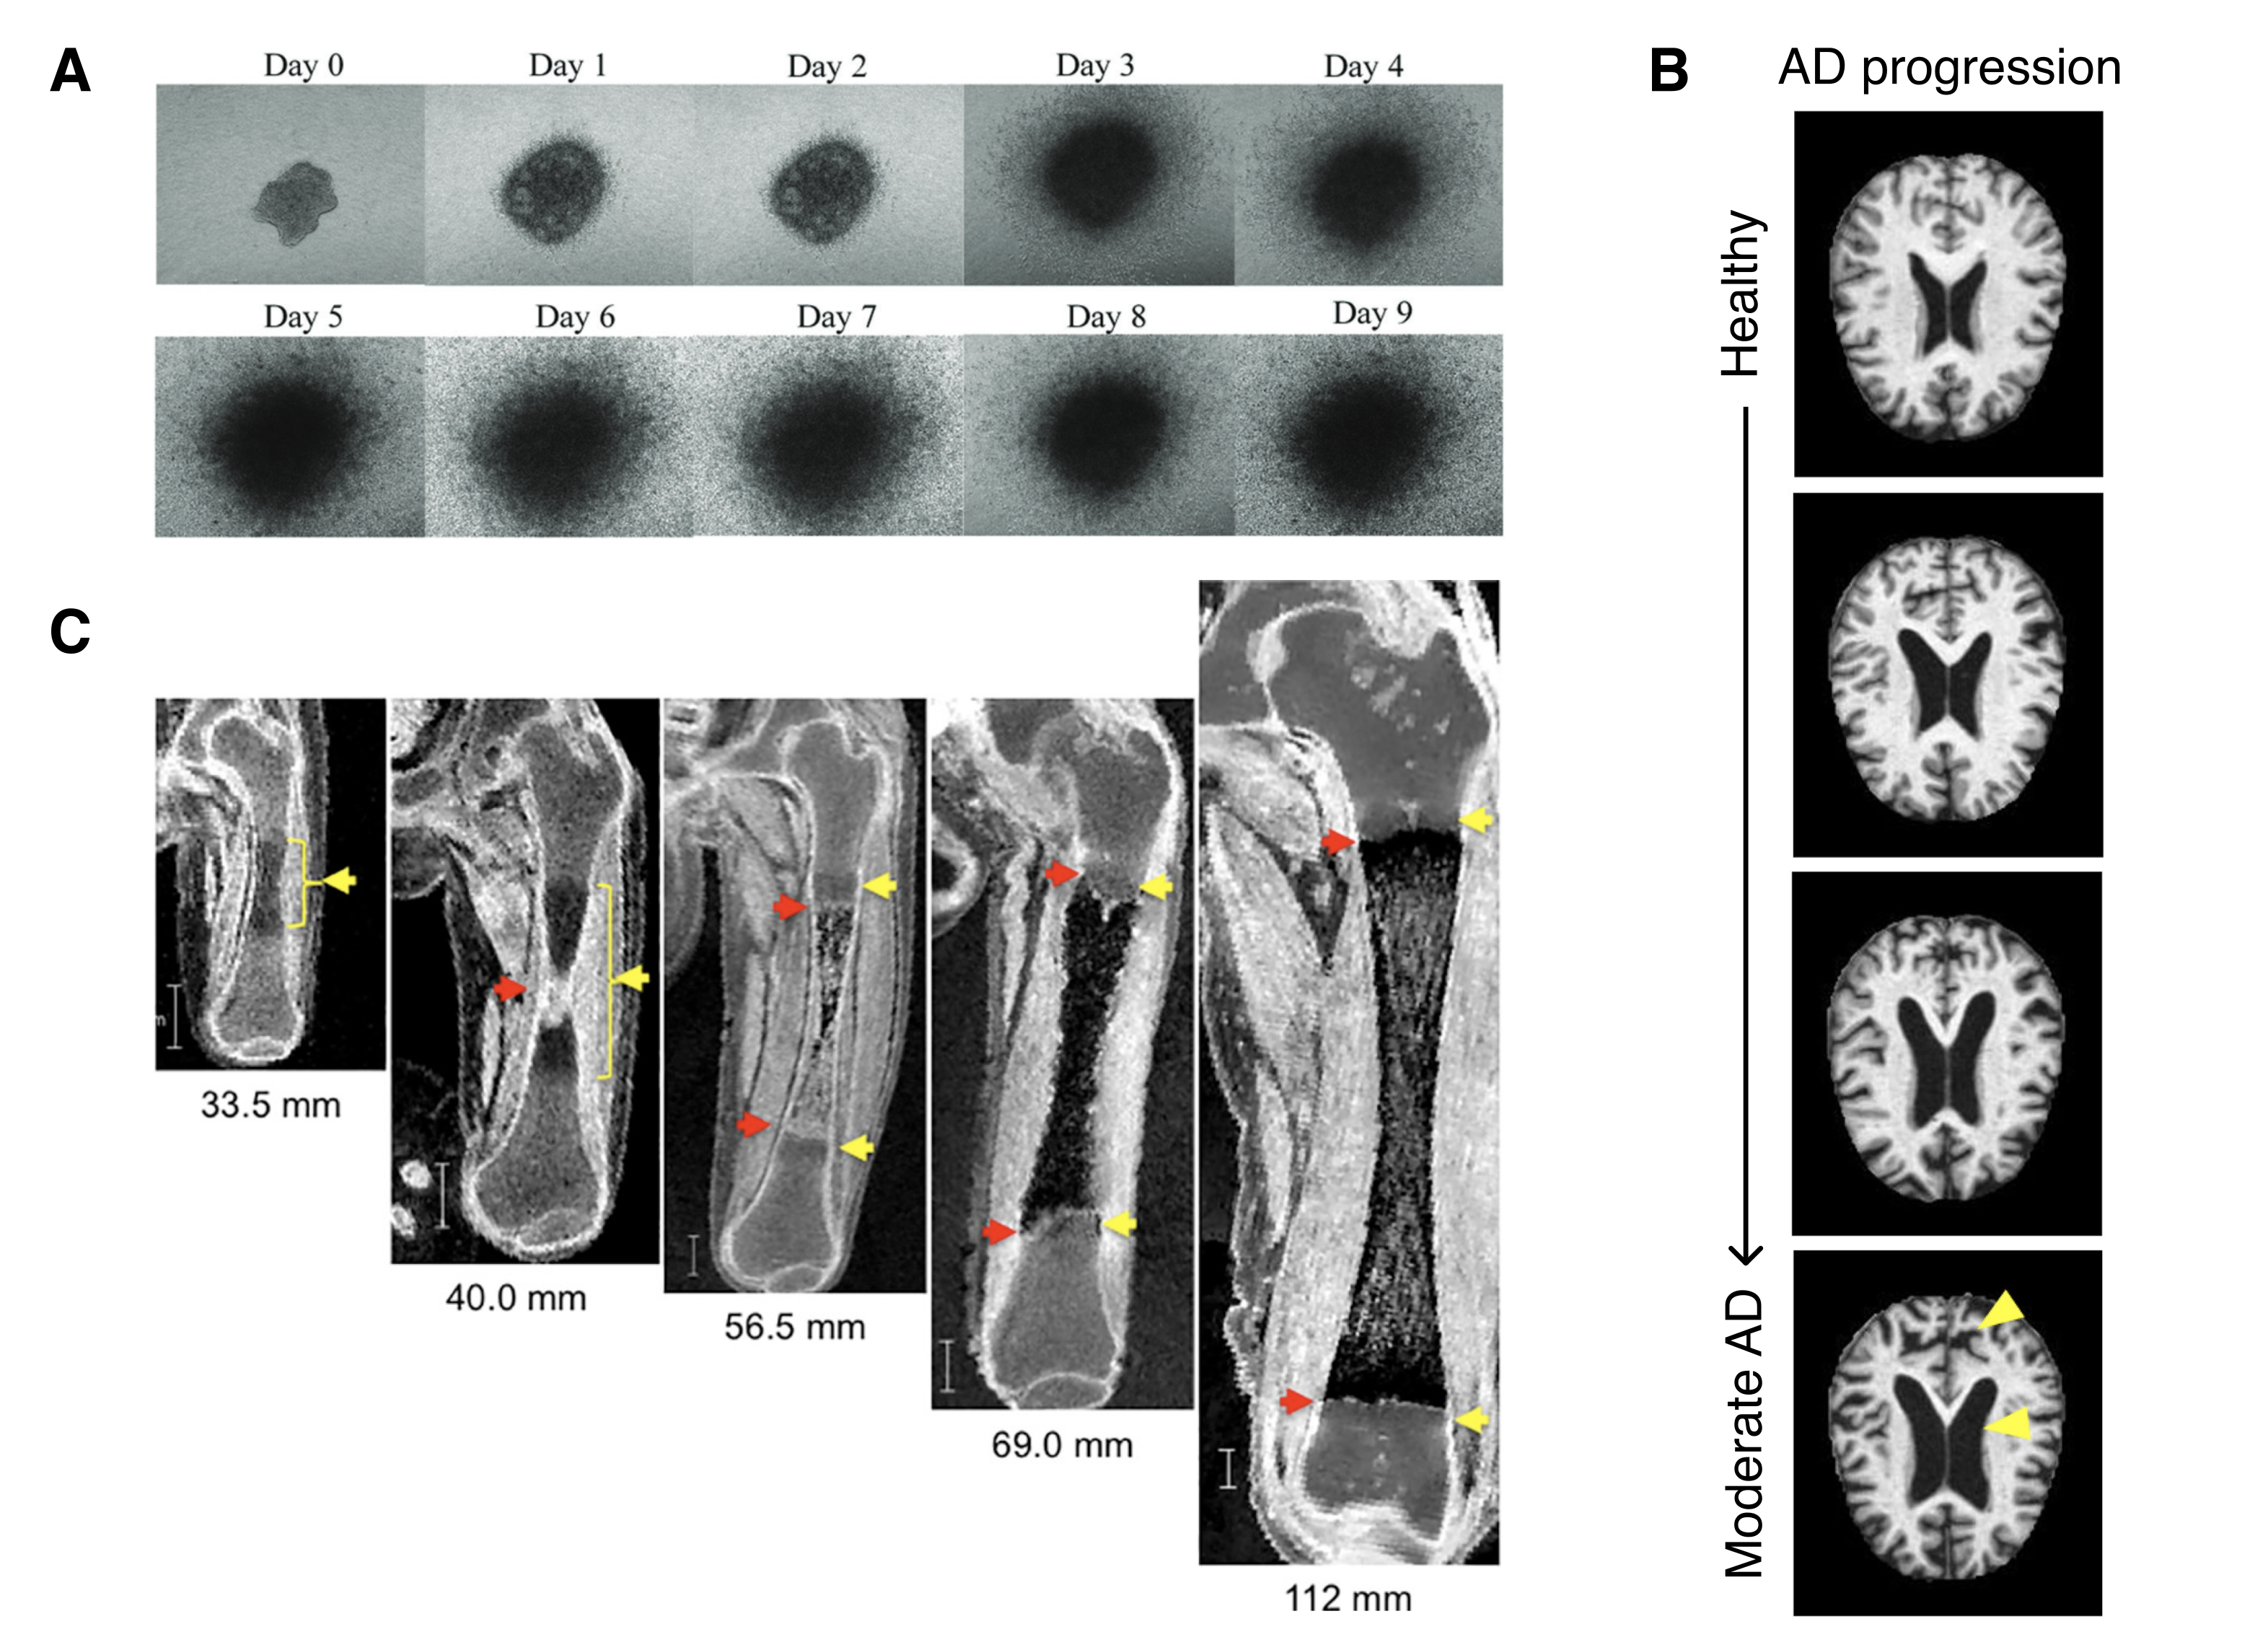
\includegraphics[scale=0.9]{fig0.png}
		\caption{\textbf{A)} Longitudinal phase contrast imaging of 3D cell cultured cervical cancer spheroids \cite{Muniandy2021}*. \textbf{B)} Neurodegradation of brain structure with progression of AD, from healthy to moderate AD (top to bottom). Adapted from \cite{Pasnoori2024}*. \textbf{C)} Longitudinal MRI imaging of the morphogenesis of a femur during the embryonic and fetal periods. Figure adapted from \cite{Suzuki2019}*. *Images obtained from referenced sources and licensed under CC BY 4.0 (https://creativecommons.org/licenses/by/4.0/)}
		\label{fig:fig0}
	\end{figure}
	\FloatBarrier		



	Early spatiotemporal shape modeling can be linked to morphometrics, wherein researchers attempted to analyze biological shape variation using statistical methods. Generally speaking, researchers analyzed variations of common anatomical landmarks across a population \cite{Slice2007}. These analyses examined variations in the coordinates of landmarks themselves, distances or relative angles between them, or metrics calculated from a combination thereof \cite{Rohlf90, Slice, 7e30a527-6aa0-3191-9009-c9d49643b4ef}. In the femur, for example, measurements such as the whole femur length, diaphyseal length, subtrochanteric anteroposterior and mediolateral diameters, anteroposterior physeal angles, alpha angle, and vertical diameter of the femoral head are some of the measurements used to characterize femoral anatomy \cite{Toogood2008, Wescott2005, Rissech2008}. These methods, however, are time-consuming and landmark placement can be unreliable, inconsistent, and fail to capture holistic spatial arrangement. Developments in computer vision and mathematical modeling tools have led to the development of computational anatomy (CA) \cite{Miller1997, Grenander1998, Miller2004}. Therein, the concept of shape manifolds and diffeomorphic transformations became central in describing anatomical shape variability over time. These tools have developed greatly in recent years. Furthermore, with the advent of deep learning (DL), novel methodologies have surfaced. Outlining available methodologies along with their strengths, weaknesses, and potential synergies is, thus, required. 

	In this review, we seek to highlight and discuss alternative techniques, methodologies, and tools used to model the changing shape of anatomical structures over time. For simplicity and due to the varied terminologies found in the literature, we use the terms spatiotemporal shape modelling and longitudinal shape models interchangeably. We also focus mainly on the techniques and tools themselves as opposed to their clinical applications. However, we highlight applications as necessary to enhance the descriptive value of the presented concepts. We also neglect exhaustive discussions on these methods' mathematical background and derivations, and instead refer the readers where necessary. Here, we refer to \textit{shape} in both a geometric sense (\textit{i.e.,} a set of points in $n$-dimensional Euclidean space ($\mathbb{R}^{n}$) with defined connections) and also in the intuitive sense of a visual boundary defining an object of interest within an image. This is important as both definitions play a role in the differing techniques we explore. A relatively similar review was carried out by Harie \textit{et al.}, however they explicitly focused on growth modeling and mainly discussed DL-based generative networks \cite{Harie2023}. In contrast, this review focuses on shape change over time in general, thus encompassing both growth and alternative biological processes (\textit{e.g.,} degeneration). Furthermore, this review does not focus exclusively on DL-based methods and also covers alternatives. This review begins with a discussion on diffeomorphisms and large deformation diffeomorphic metric mapping (LDDMM) framework, the most common early framework for spatiotemporal shape modeling. Then, we discuss deep learning-based tools, focusing on autoencoders, generative adversarial networks, recurrent neural networks, and transformers. Finally, we discuss the strengths and drawbacks of each tool generally, highlighting similarities and potential synergies. We also speculate on potential future outlooks and directions for research into spatiotemporal shape modelling. 
	